\section{Propriet\`a Specifiche}
\label{sec:chapter_3_section_3}

\noindent

Ogni plugin ha una serie di proprietà specifiche degli elementi costruttivi che rappresenta.
Ogni propriet\`a \`e definita da:
\begin{itemize}
  \item un \emph{name};
  \item un \emph{type} (come ``number'', ``text'', ``boolean'', o ``custom'');
  \item un \emph{value}.
\end{itemize}
In accordo con il proprio tipo, ciascun valore di ogni proprietà presenta un interfaccia dedicata per l'inserimento dei valori.
Ad esempio, un valore della proprietà booleana è impostato tramite una casella di controllo (checkbox),
mentre una proprietà di testo è inserita attraverso una casella di testo (Figura~\ref{fig:dettaglio}).

\begin{figure}[htbp] %  figure placement: here, top, bottom, or page
   \centering
   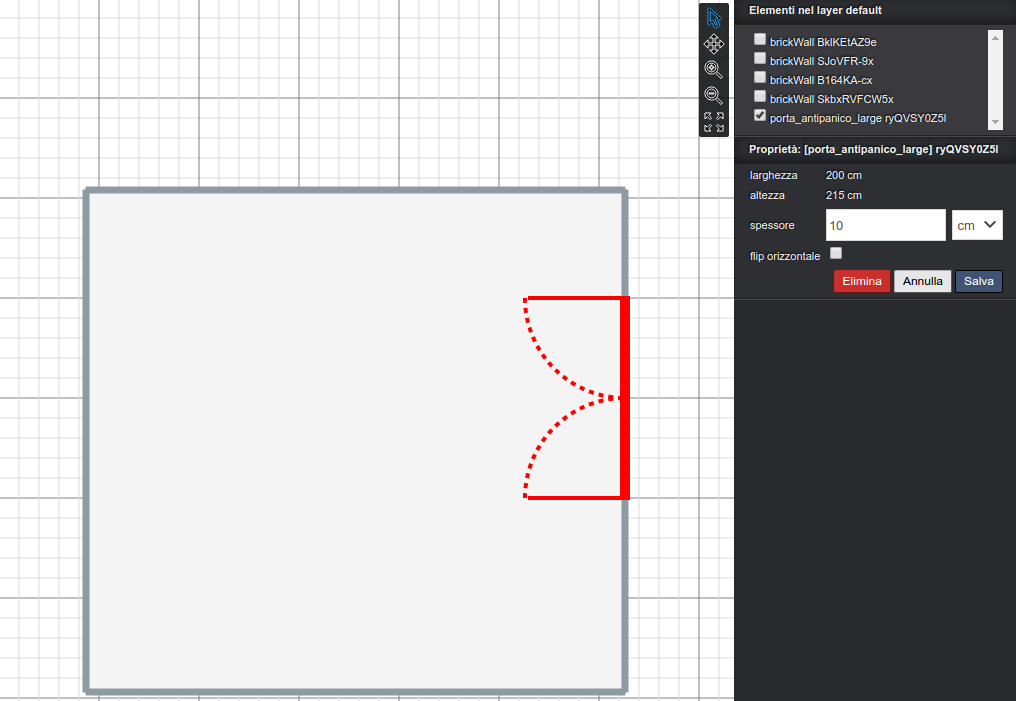
\includegraphics[width=1\linewidth]{images/dettaglio}
   \caption{Esempio sidebar con checkbox e casella di testo}
   \label{fig:dettaglio}
   \end{figure}
\newpage

Il sistema \`e progettato per accettare tipi di propriet\`a custom. Un propriet\`a custom è richiesta per definire
il componente della UI che permette all'utente di inserire il suo valore.
Per esempio, una propriet\`a ``colore'' pu\`o essere introdotta definendo un componente della UI composto da tre box di testo
(ad esempio per ogni componente RGB), mentre una propriet\`a ``length'' pu\`o essere introdotta definendo un componente UI
includendo una box di testo per il valore e menu drop-down per le unità di misura.

Le propriet\`a specifiche di un elemento possono essere modificate nel relativo pannello nella sidebar, una volta che l'elemento
\`e stato selezionato nel content-area.
\newpage
